% Этот шаблон документа разработан в 2014 году
% Данилом Фёдоровых (danil@fedorovykh.ru) 
% для использования в курсе 
% <<Документы и презентации в \LaTeX>>, записанном НИУ ВШЭ
% для Coursera.org: http://coursera.org/course/latex .
% Исходная версия шаблона --- 
% https://www.writelatex.com/coursera/latex/2

\documentclass[a4paper,12pt]{article}

%%% Работа с русским языком
\usepackage{cmap}					% поиск в PDF
\usepackage{mathtext} 				% русские буквы в фомулах
\usepackage[T2A]{fontenc}			% кодировка
\usepackage[utf8]{inputenc}			% кодировка исходного текста
\usepackage[english,russian]{babel}	% локализация и переносы

%%% Дополнительная работа с математикой
\usepackage{amsfonts,amssymb,amsthm,mathtools} % AMS
\usepackage{amsmath}
\usepackage{icomma} % "Умная" запятая: $0,2$ --- число, $0, 2$ --- перечисление

%% Номера формул
%\mathtoolsset{showonlyrefs=true} % Показывать номера только у тех формул, на которые есть \eqref{} в тексте.

%% Шрифты
\usepackage{euscript}	 % Шрифт Евклид
\usepackage{mathrsfs} % Красивый матшрифт

%% Свои команды
\DeclareMathOperator{\sgn}{\mathop{sgn}}

%% Перенос знаков в формулах (по Львовскому)
\newcommand*{\hm}[1]{#1\nobreak\discretionary{}
{\hbox{$\mathsurround=0pt #1$}}{}}

%%% Работа с картинками
\usepackage{graphicx}  % Для вставки рисунков
\graphicspath{{images/}{images2/}}  % папки с картинками
\setlength\fboxsep{3pt} % Отступ рамки \fbox{} от рисунка
\setlength\fboxrule{1pt} % Толщина линий рамки \fbox{}
\usepackage{wrapfig} % Обтекание рисунков и таблиц текстом

%%% Работа с таблицами
\usepackage{array,tabularx,tabulary,booktabs} % Дополнительная работа с таблицами
\usepackage{longtable}  % Длинные таблицы
\usepackage{multirow} % Слияние строк в таблице


%%% Заголовок
\author{Документы и презентации в \LaTeX}
\title{2.1 Рисунки и таблицы}
\date{\today}

\begin{document} % конец преамбулы, начало документа

\maketitle

\section{Картинки}

\subsection{Растровые рисунки}

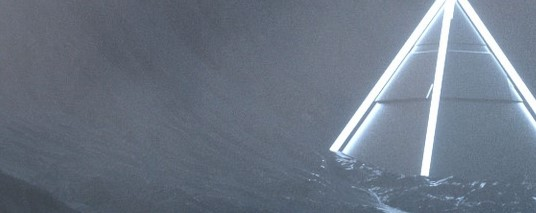
\includegraphics{znak.jpg}

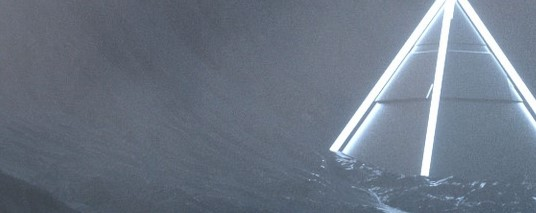
\includegraphics[scale=2]{znak.jpg}

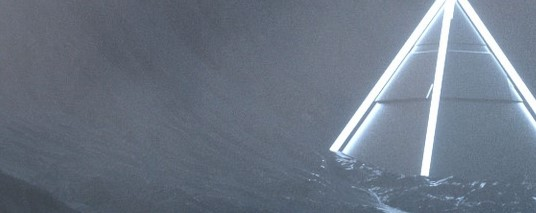
\includegraphics[width=10cm,height=7cm,keepaspectratio]{znak.jpg}

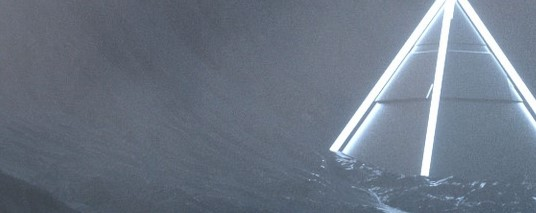
\includegraphics[draft]{znak.jpg}

\subsection{Векторные картинки}

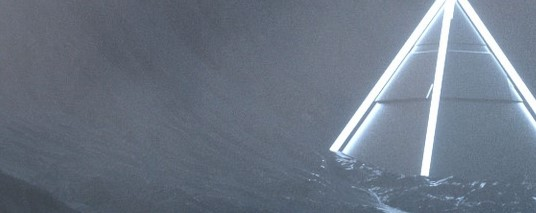
\includegraphics[width=\textwidth]{znak.jpg}

\section{Таблицы}

\begin{tabular}{|p{4cm}cp{5cm}|}
	\hline
	Это очень-очень длинное предложение из многих слов. & $6\times 2$ &  Это очень-очень длинное предложение из многих слов. \\ 
	\hline
	21 & $\displaystyle \frac{x}{y}$ & 23  \\
	\hline
	31 & 32 & 33 \\ 
	\hline 
\end{tabular} 

\begin{tabularx}{\textwidth}{X|c|X}
	\hline
	Это очень-очень длинное предложение из многих слов & Текст покороче & Это очень-очень длинное предложение из многих слов Это очень-очень длинное предложение из многих слов
\end{tabularx}


\begin{tabulary}{\textwidth}{C|J|R}
	\hline
	Это очень-очень длинное предложение из многих слов & Текст покороче & Это очень-очень длинное предложение из многих слов Это очень-очень длинное предложение из многих слов
\end{tabulary}

\section{Плавающие объекты}

Смотри таблицу \ref{tab:mytab}.

\begin{table}[!h]
	\begin{center}
		\caption[Заголовок для списка таблиц]{Бессмысленная таблица, зато с кучей фишек.}\label{tab:mytab}
		\begin{tabular}{|c|c|c|c||l|c|c|r|c|c|}
  		\hline
    	1 & 2 & 3 & 4 & 5 & 6 & 7 & 8 & 9 & 10 \\ \hline
  		Первый & Второй & \multicolumn{3}{|c|}{Третий -- пятый} &   &  & Восьмой &   &  \\ 
		\cline{1-7} \cline{9-10}
   		1 & 2 & 3 & 4 & 5 & 6 & 7 & 8 & 9 & 10 \\ \hline \hline
   		1 & 2 & 3 & 4 & 5 & 6 & 7 & 8 & 9 & 10 \\ \hline
    	\multirow{3}{*}{Три строки}  & 2 & 3 & 4 & 5 & 6 & 7 & 8 & 9 & 10 \\ \cline{2-10}
    	  & 2 & 3 & 4 & 5 & 6 & 7 & 8 & 9 & 10 \\ \cline{2-10}
    	  & 2 & 3 & 4 & 5 & 6 & 7 & 8 & 9 & 10 \\ \hline
		\end{tabular}
	\end{center}
	%\caption{Заголовок мог быть и здесь}
\end{table}




\begin{longtable}{|c|c|c|c|}
	\caption{Заголовок большой таблицы.}\\
	\hline
	\textbf{RND1} & \textbf{RND2} & \textbf{RND3} & \textbf{RND4} \\ \hline
	\endfirsthead
	\hline
	RND1 & RND2 & RND3 & RND4 \\ \hline
	\endhead
	\hline
	\multicolumn{4}{r}{продолжение следует\ldots} \
	\endfoot
	\hline
	\endlastfoot

0,576745371 & 0,435853468 & 0,36384912 & 0,299047979 \\ 
0,064795364 & 0,028454613 & 0,751312059 & 0,693972684 \\
0,263563971 & 0,367508634 & 0,075536384 & 0,337780707 \\
0,957583964 & 0,431948588 & 0,938522377 & 0,464307785 \\
0,815740484 & 0,123129806 & 0,883432767 & 0,760983283 \\
0,445062335 & 0,157424268 & 0,883442259 & 0,300596338 \\
0,187159669 & 0,728663343 & 0,637199982 & 0,765684528 \\
0,41009848 & 0,457031472 & 0,142858106 & 0,602946607 \\
0,43315663 & 0,26058316 & 0,611667007 & 0,400328185 \\
0,824086963 & 0,27304335 & 0,244565296 & 0,219675484 \\
0,109578811 & 0,278478018 & 0,242519359 & 0,414669471 \\
0,220778432 & 0,938106645 & 0,502630894 & 0,910760406 \\
0,905239004 & 0,017835419 & 0,429423867 & 0,299079986 \\
0,604679988 & 0,784786124 & 0,86825382 & 0,003631105 \\
0,725883239 & 0,273875543 & 0,843605984 & 0,607743466 \\
0,555736787 & 0,019487901 & 0,342950631 & 0,537183422 \\
0,309374962 & 0,44331087 & 0,749656403 & 0,966836051 \\
0,274332831 & 0,740197878 & 0,865450742 & 0,792816484 \\
0,968626843 & 0,580215733 & 0,706427331 & 0,879562225 \\
0,281344607 & 0,51362826 & 0,7998827 & 0,270290356 \\
0,885143961 & 0,989455756 & 0,235591368 & 0,693434397 \\
0,505067377 & 0,127308502 & 0,614625825 & 0,277375342 \\
0,663594497 & 0,023550761 & 0,670822594 & 0,302446663 \\
0,094723947 & 0,091199224 & 0,841117852 & 0,617394243 \\
0,490246305 & 0,761569651 & 0,973576975 & 0,51597127 \\
0,631301873 & 0,155944248 & 0,319958965 & 0,198643097 \\
0,853761692 & 0,993889567 & 0,105045533 & 0,837805396 \\
0,149834425 & 0,316419619 & 0,387770251 & 0,552013475 \\
0,269182006 & 0,721020214 & 0,484218147 & 0,552132834 \\
0,668632873 & 0,699511389 & 0,278877959 & 0,021775345 \\
0,62638369 & 0,737702261 & 0,696351048 & 0,256427487 \\
0,922563692 & 0,629514529 & 0,789891184 & 0,019748079 \\
0,366649518 & 0,882085214 & 0,805771543 & 0,461659364 \\
0,178967822 & 0,400706498 & 0,313063544 & 0,425676173 \\
0,328582166 & 0,124008134 & 0,177734655 & 0,653821253 \\
0,318628436 & 0,924056157 & 0,005170407 & 0,09988244 \\
0,1523348 & 0,686022531 & 0,877786704 & 0,230997696 \\
0,160048577 & 0,475334591 & 0,118018156 & 0,720594848 \\
0,502602506 & 0,898504748 & 0,103602236 & 0,289059862 \\
0,185262766 & 0,640333509 & 0,980932923 & 0,424269289 \\
0,63740761 & 0,665837647 & 0,256564927 & 0,796877433 \\
0,326795292 & 0,863892719 & 0,19537989 & 0,410369904 \\
0,377332846 & 0,61459335 & 0,158101373 & 0,100684292 \\
0,540188499 & 0,911708617 & 0,077277867 & 0,108818241 \\
0,485200234 & 0,692007154 & 0,012528805 & 0,364692863 \\
0,435947515 & 0,555444136 & 0,410076838 & 0,973027822 \\
0,423053661 & 0,502696027 & 0,500150945 & 0,209929767 \\
0,146604488 & 0,318962234 & 0,535025906 & 0,25597358 \\
0,252933039 & 0,897587117 & 0,961039174 & 0,238301151 \\
0,798559806 & 0,885674601 & 0,451623639 & 0,903044881 \\
0,467795852 & 0,398491485 & 0,09863235 & 0,110588673 \\
0,932456386 & 0,679931054 & 0,499049066 & 0,419347908 \\
0,806742814 & 0,998944815 & 0,730738513 & 0,207088322 \\
0,524028453 & 0,251332909 & 0,711910448 & 0,243583774 \\
0,037417208 & 0,333822686 & 0,276647434 & 0,882818666 \\
0,358649112 & 0,534662608 & 0,726203191 & 0,041117785 \\
0,141309914 & 0,36643456 & 0,552053605 & 0,956487966 \\
0,53808496 & 0,939874695 & 0,186724749 & 0,690302117 \\
0,052101497 & 0,887611776 & 0,677925016 & 0,622234766 \\
0,553154653 & 0,040281685 & 0,504952332 & 0,097544063 \\
0,732288281 & 0,658739311 & 0,883348524 & 0,144957902 \\
0,288649747 & 0,517727905 & 0,639432157 & 0,456739615 \\
0,293369191 & 0,138002629 & 0,154228354 & 0,133189564 \\
0,693221668 & 0,246693033 & 0,465542044 & 0,978720597 \\
0,135587928 & 0,15068455 & 0,825417066 & 0,885949167 \\
0,676052335 & 0,253724745 & 0,219361854 & 0,808580891 \\
0,582461065 & 0,554730526 & 0,476287005 & 0,268673107 \\
0,238129516 & 0,090469211 & 0,525167086 & 0,59620778 \\
0,769704124 & 0,27036399 & 0,888763617 & 0,089602751 \\
0,548435183 & 0,357753532 & 0,858061896 & 0,465681708 \\
0,702731358 & 0,856923488 & 0,058935386 & 0,675796794 \\
0,338117119 & 0,622858325 & 0,461848295 & 0,94572588 \\
0,606619551 & 0,999527337 & 0,361750308 & 0,673771858 \\
0,221137745 & 0,719189979 & 0,624447286 & 0,59032258 \\
0,239784727 & 0,636404041 & 0,841898027 & 0,844823258 \\
0,800614467 & 0,368896918 & 0,994129014 & 0,291457496 \\
0,681757552 & 0,019367985 & 0,417601531 & 0,649347809 \\
0,28051889 & 0,061635488 & 0,914332594 & 0,331713964 \\
0,657743996 & 0,983965656 & 0,818946725 & 0,36394332 \\
0,543479307 & 0,169289586 & 0,483196672 & 0,985172369 \\
0,145081556 & 0,892455096 & 0,190462767 & 0,824433551 \\
0,196973955 & 0,995308839 & 0,879891823 & 0,845636911 \\
0,904947195 & 0,593928658 & 0,403422613 & 0,076252813 \\
0,269580321 & 0,740772576 & 0,182364329 & 0,695081896 \\
0,293711052 & 0,351494187 & 0,331350034 & 0,62158188 \\
0,69779066 & 0,019424915 & 0,657473072 & 0,783698296 \\
0,14204222 & 0,817006985 & 0,669234791 & 0,728306309 \\
0,38941124 & 0,807135743 & 0,702842593 & 0,382494957 \\
0,203543688 & 0,969191131 & 0,822881425 & 0,212473701 \\
0,826623142 & 0,181291269 & 0,054701556 & 0,386442059 \\
0,541365118 & 0,573617788 & 0,650112336 & 0,930417614 \\
0,277453725 & 0,382833978 & 0,395547164 & 0,785051981 \\
0,078149646 & 0,115526198 & 0,417197235 & 0,894812516 \\
0,772854891 & 0,698024923 & 0,504995217 & 0,492422679 \\
0,592288285 & 0,153957871 & 0,348784682 & 0,523821625 \\
0,618156868 & 0,841905787 & 0,038053593 & 0,861496223 \\
0,76387049 & 0,652733723 & 0,034948244 & 0,814496925 \\
\end{longtable}

\begin{wrapfigure}{l}{0.3333\linewidth}
	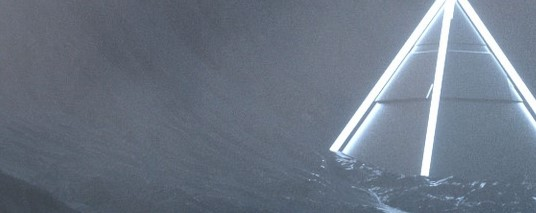
\includegraphics[width=\linewidth]{znak.jpg}
	\caption{Картинка с обтеканием}
\end{wrapfigure}Распоряжением Правительства Российской Федерации от 12 августа 2008 г. ВШЭ перешла в ведение Правительства РФ. До 12 августа 2008 г. ВШЭ находилась в ведении Министерства экономического развития и торговли РФ.

Решением конкурсной комиссии Министерства образования и науки РФ от 7 октября 2009 года в отношении ВШЭ установлена категория "национальный исследовательский университет". 

Постановлением Правительства РФ от 23 декабря 2010 года № 1109 «О создании федерального государственного автономного образовательного учреждения высшего профессионального образования «Национальный исследовательский университет «Высшая школа экономики» университет получил новое название и статус автономного образовательного учреждения. До 23 декабря 2010 года университет носил официальное название ГУ-ВШЭ.

\begin{wraptable}{r}{0.5\linewidth}
		\begin{tabular}{|c|c|c|c|c|c|}
			\hline
			Год & $P_x$ &$Q_x$ & $P_y$ & $Q_y$ & $n$\\ \hline
			2008 &  & 36 &  & 32 & — \\ \hline
			2009 & 30 & 30 & 22 & 50 & 25 \% \\ \hline
			2010 & 36 & 30 & 22 &  & 20 \% \\ \hline
			2011 & 33 & 40 & 24 & 45 & \\ \hline
		\end{tabular}
		\caption{Обтекаемая таблица}
\end{wraptable}Распоряжением Правительства Российской Федерации от 12 августа 2008 г. ВШЭ перешла в ведение Правительства РФ. До 12 августа 2008 г. ВШЭ находилась в ведении Министерства экономического развития и торговли РФ.

Решением конкурсной комиссии Министерства образования и науки РФ от 7 октября 2009 года в отношении ВШЭ установлена категория "национальный исследовательский университет". 

Постановлением Правительства РФ от 23 декабря 2010 года № 1109 «О создании федерального государственного автономного образовательного учреждения высшего профессионального образования «Национальный исследовательский университет «Высшая школа экономики» университет получил новое название и статус автономного образовательного учреждения. До 23 декабря 2010 года университет носил официальное название ГУ-ВШЭ.

\listoffigures

\listoftables

\end{document} % конец документа

